\documentclass[11pt]{article}

    \usepackage[breakable]{tcolorbox}
    \usepackage{parskip} % Stop auto-indenting (to mimic markdown behaviour)
    

    % Basic figure setup, for now with no caption control since it's done
    % automatically by Pandoc (which extracts ![](path) syntax from Markdown).
    \usepackage{graphicx}
    % Keep aspect ratio if custom image width or height is specified
    \setkeys{Gin}{keepaspectratio}
    % Maintain compatibility with old templates. Remove in nbconvert 6.0
    \let\Oldincludegraphics\includegraphics
    % Ensure that by default, figures have no caption (until we provide a
    % proper Figure object with a Caption API and a way to capture that
    % in the conversion process - todo).
    \usepackage{caption}
    \DeclareCaptionFormat{nocaption}{}
    \captionsetup{format=nocaption,aboveskip=0pt,belowskip=0pt}

    \usepackage{float}
    \floatplacement{figure}{H} % forces figures to be placed at the correct location
    \usepackage{xcolor} % Allow colors to be defined
    \usepackage{enumerate} % Needed for markdown enumerations to work
    \usepackage{geometry} % Used to adjust the document margins
    \usepackage{amsmath} % Equations
    \usepackage{amssymb} % Equations
    \usepackage{textcomp} % defines textquotesingle
    % Hack from http://tex.stackexchange.com/a/47451/13684:
    \AtBeginDocument{%
        \def\PYZsq{\textquotesingle}% Upright quotes in Pygmentized code
    }
    \usepackage{upquote} % Upright quotes for verbatim code
    \usepackage{eurosym} % defines \euro

    \usepackage{iftex}
    \ifPDFTeX
        \usepackage[T1]{fontenc}
        \IfFileExists{alphabeta.sty}{
              \usepackage{alphabeta}
          }{
              \usepackage[mathletters]{ucs}
              \usepackage[utf8x]{inputenc}
          }
    \else
        \usepackage{fontspec}
        \usepackage{unicode-math}
    \fi

    \usepackage{fancyvrb} % verbatim replacement that allows latex
    \usepackage{grffile} % extends the file name processing of package graphics
                         % to support a larger range
    \makeatletter % fix for old versions of grffile with XeLaTeX
    \@ifpackagelater{grffile}{2019/11/01}
    {
      % Do nothing on new versions
    }
    {
      \def\Gread@@xetex#1{%
        \IfFileExists{"\Gin@base".bb}%
        {\Gread@eps{\Gin@base.bb}}%
        {\Gread@@xetex@aux#1}%
      }
    }
    \makeatother
    \usepackage[Export]{adjustbox} % Used to constrain images to a maximum size
    \adjustboxset{max size={0.9\linewidth}{0.9\paperheight}}

    % The hyperref package gives us a pdf with properly built
    % internal navigation ('pdf bookmarks' for the table of contents,
    % internal cross-reference links, web links for URLs, etc.)
    \usepackage{hyperref}
    % The default LaTeX title has an obnoxious amount of whitespace. By default,
    % titling removes some of it. It also provides customization options.
    \usepackage{titling}
    \usepackage{longtable} % longtable support required by pandoc >1.10
    \usepackage{booktabs}  % table support for pandoc > 1.12.2
    \usepackage{array}     % table support for pandoc >= 2.11.3
    \usepackage{calc}      % table minipage width calculation for pandoc >= 2.11.1
    \usepackage[inline]{enumitem} % IRkernel/repr support (it uses the enumerate* environment)
    \usepackage[normalem]{ulem} % ulem is needed to support strikethroughs (\sout)
                                % normalem makes italics be italics, not underlines
    \usepackage{soul}      % strikethrough (\st) support for pandoc >= 3.0.0
    \usepackage{mathrsfs}
    

    
    % Colors for the hyperref package
    \definecolor{urlcolor}{rgb}{0,.145,.698}
    \definecolor{linkcolor}{rgb}{.71,0.21,0.01}
    \definecolor{citecolor}{rgb}{.12,.54,.11}

    % ANSI colors
    \definecolor{ansi-black}{HTML}{3E424D}
    \definecolor{ansi-black-intense}{HTML}{282C36}
    \definecolor{ansi-red}{HTML}{E75C58}
    \definecolor{ansi-red-intense}{HTML}{B22B31}
    \definecolor{ansi-green}{HTML}{00A250}
    \definecolor{ansi-green-intense}{HTML}{007427}
    \definecolor{ansi-yellow}{HTML}{DDB62B}
    \definecolor{ansi-yellow-intense}{HTML}{B27D12}
    \definecolor{ansi-blue}{HTML}{208FFB}
    \definecolor{ansi-blue-intense}{HTML}{0065CA}
    \definecolor{ansi-magenta}{HTML}{D160C4}
    \definecolor{ansi-magenta-intense}{HTML}{A03196}
    \definecolor{ansi-cyan}{HTML}{60C6C8}
    \definecolor{ansi-cyan-intense}{HTML}{258F8F}
    \definecolor{ansi-white}{HTML}{C5C1B4}
    \definecolor{ansi-white-intense}{HTML}{A1A6B2}
    \definecolor{ansi-default-inverse-fg}{HTML}{FFFFFF}
    \definecolor{ansi-default-inverse-bg}{HTML}{000000}

    % common color for the border for error outputs.
    \definecolor{outerrorbackground}{HTML}{FFDFDF}

    % commands and environments needed by pandoc snippets
    % extracted from the output of `pandoc -s`
    \providecommand{\tightlist}{%
      \setlength{\itemsep}{0pt}\setlength{\parskip}{0pt}}
    \DefineVerbatimEnvironment{Highlighting}{Verbatim}{commandchars=\\\{\}}
    % Add ',fontsize=\small' for more characters per line
    \newenvironment{Shaded}{}{}
    \newcommand{\KeywordTok}[1]{\textcolor[rgb]{0.00,0.44,0.13}{\textbf{{#1}}}}
    \newcommand{\DataTypeTok}[1]{\textcolor[rgb]{0.56,0.13,0.00}{{#1}}}
    \newcommand{\DecValTok}[1]{\textcolor[rgb]{0.25,0.63,0.44}{{#1}}}
    \newcommand{\BaseNTok}[1]{\textcolor[rgb]{0.25,0.63,0.44}{{#1}}}
    \newcommand{\FloatTok}[1]{\textcolor[rgb]{0.25,0.63,0.44}{{#1}}}
    \newcommand{\CharTok}[1]{\textcolor[rgb]{0.25,0.44,0.63}{{#1}}}
    \newcommand{\StringTok}[1]{\textcolor[rgb]{0.25,0.44,0.63}{{#1}}}
    \newcommand{\CommentTok}[1]{\textcolor[rgb]{0.38,0.63,0.69}{\textit{{#1}}}}
    \newcommand{\OtherTok}[1]{\textcolor[rgb]{0.00,0.44,0.13}{{#1}}}
    \newcommand{\AlertTok}[1]{\textcolor[rgb]{1.00,0.00,0.00}{\textbf{{#1}}}}
    \newcommand{\FunctionTok}[1]{\textcolor[rgb]{0.02,0.16,0.49}{{#1}}}
    \newcommand{\RegionMarkerTok}[1]{{#1}}
    \newcommand{\ErrorTok}[1]{\textcolor[rgb]{1.00,0.00,0.00}{\textbf{{#1}}}}
    \newcommand{\NormalTok}[1]{{#1}}

    % Additional commands for more recent versions of Pandoc
    \newcommand{\ConstantTok}[1]{\textcolor[rgb]{0.53,0.00,0.00}{{#1}}}
    \newcommand{\SpecialCharTok}[1]{\textcolor[rgb]{0.25,0.44,0.63}{{#1}}}
    \newcommand{\VerbatimStringTok}[1]{\textcolor[rgb]{0.25,0.44,0.63}{{#1}}}
    \newcommand{\SpecialStringTok}[1]{\textcolor[rgb]{0.73,0.40,0.53}{{#1}}}
    \newcommand{\ImportTok}[1]{{#1}}
    \newcommand{\DocumentationTok}[1]{\textcolor[rgb]{0.73,0.13,0.13}{\textit{{#1}}}}
    \newcommand{\AnnotationTok}[1]{\textcolor[rgb]{0.38,0.63,0.69}{\textbf{\textit{{#1}}}}}
    \newcommand{\CommentVarTok}[1]{\textcolor[rgb]{0.38,0.63,0.69}{\textbf{\textit{{#1}}}}}
    \newcommand{\VariableTok}[1]{\textcolor[rgb]{0.10,0.09,0.49}{{#1}}}
    \newcommand{\ControlFlowTok}[1]{\textcolor[rgb]{0.00,0.44,0.13}{\textbf{{#1}}}}
    \newcommand{\OperatorTok}[1]{\textcolor[rgb]{0.40,0.40,0.40}{{#1}}}
    \newcommand{\BuiltInTok}[1]{{#1}}
    \newcommand{\ExtensionTok}[1]{{#1}}
    \newcommand{\PreprocessorTok}[1]{\textcolor[rgb]{0.74,0.48,0.00}{{#1}}}
    \newcommand{\AttributeTok}[1]{\textcolor[rgb]{0.49,0.56,0.16}{{#1}}}
    \newcommand{\InformationTok}[1]{\textcolor[rgb]{0.38,0.63,0.69}{\textbf{\textit{{#1}}}}}
    \newcommand{\WarningTok}[1]{\textcolor[rgb]{0.38,0.63,0.69}{\textbf{\textit{{#1}}}}}
    \makeatletter
    \newsavebox\pandoc@box
    \newcommand*\pandocbounded[1]{%
      \sbox\pandoc@box{#1}%
      % scaling factors for width and height
      \Gscale@div\@tempa\textheight{\dimexpr\ht\pandoc@box+\dp\pandoc@box\relax}%
      \Gscale@div\@tempb\linewidth{\wd\pandoc@box}%
      % select the smaller of both
      \ifdim\@tempb\p@<\@tempa\p@
        \let\@tempa\@tempb
      \fi
      % scaling accordingly (\@tempa < 1)
      \ifdim\@tempa\p@<\p@
        \scalebox{\@tempa}{\usebox\pandoc@box}%
      % scaling not needed, use as it is
      \else
        \usebox{\pandoc@box}%
      \fi
    }
    \makeatother

    % Define a nice break command that doesn't care if a line doesn't already
    % exist.
    \def\br{\hspace*{\fill} \\* }
    % Math Jax compatibility definitions
    \def\gt{>}
    \def\lt{<}
    \let\Oldtex\TeX
    \let\Oldlatex\LaTeX
    \renewcommand{\TeX}{\textrm{\Oldtex}}
    \renewcommand{\LaTeX}{\textrm{\Oldlatex}}
    % Document parameters
    % Document title
    \title{12\_notes}
    
    
    
    
    
    
    
% Pygments definitions
\makeatletter
\def\PY@reset{\let\PY@it=\relax \let\PY@bf=\relax%
    \let\PY@ul=\relax \let\PY@tc=\relax%
    \let\PY@bc=\relax \let\PY@ff=\relax}
\def\PY@tok#1{\csname PY@tok@#1\endcsname}
\def\PY@toks#1+{\ifx\relax#1\empty\else%
    \PY@tok{#1}\expandafter\PY@toks\fi}
\def\PY@do#1{\PY@bc{\PY@tc{\PY@ul{%
    \PY@it{\PY@bf{\PY@ff{#1}}}}}}}
\def\PY#1#2{\PY@reset\PY@toks#1+\relax+\PY@do{#2}}

\@namedef{PY@tok@w}{\def\PY@tc##1{\textcolor[rgb]{0.73,0.73,0.73}{##1}}}
\@namedef{PY@tok@c}{\let\PY@it=\textit\def\PY@tc##1{\textcolor[rgb]{0.24,0.48,0.48}{##1}}}
\@namedef{PY@tok@cp}{\def\PY@tc##1{\textcolor[rgb]{0.61,0.40,0.00}{##1}}}
\@namedef{PY@tok@k}{\let\PY@bf=\textbf\def\PY@tc##1{\textcolor[rgb]{0.00,0.50,0.00}{##1}}}
\@namedef{PY@tok@kp}{\def\PY@tc##1{\textcolor[rgb]{0.00,0.50,0.00}{##1}}}
\@namedef{PY@tok@kt}{\def\PY@tc##1{\textcolor[rgb]{0.69,0.00,0.25}{##1}}}
\@namedef{PY@tok@o}{\def\PY@tc##1{\textcolor[rgb]{0.40,0.40,0.40}{##1}}}
\@namedef{PY@tok@ow}{\let\PY@bf=\textbf\def\PY@tc##1{\textcolor[rgb]{0.67,0.13,1.00}{##1}}}
\@namedef{PY@tok@nb}{\def\PY@tc##1{\textcolor[rgb]{0.00,0.50,0.00}{##1}}}
\@namedef{PY@tok@nf}{\def\PY@tc##1{\textcolor[rgb]{0.00,0.00,1.00}{##1}}}
\@namedef{PY@tok@nc}{\let\PY@bf=\textbf\def\PY@tc##1{\textcolor[rgb]{0.00,0.00,1.00}{##1}}}
\@namedef{PY@tok@nn}{\let\PY@bf=\textbf\def\PY@tc##1{\textcolor[rgb]{0.00,0.00,1.00}{##1}}}
\@namedef{PY@tok@ne}{\let\PY@bf=\textbf\def\PY@tc##1{\textcolor[rgb]{0.80,0.25,0.22}{##1}}}
\@namedef{PY@tok@nv}{\def\PY@tc##1{\textcolor[rgb]{0.10,0.09,0.49}{##1}}}
\@namedef{PY@tok@no}{\def\PY@tc##1{\textcolor[rgb]{0.53,0.00,0.00}{##1}}}
\@namedef{PY@tok@nl}{\def\PY@tc##1{\textcolor[rgb]{0.46,0.46,0.00}{##1}}}
\@namedef{PY@tok@ni}{\let\PY@bf=\textbf\def\PY@tc##1{\textcolor[rgb]{0.44,0.44,0.44}{##1}}}
\@namedef{PY@tok@na}{\def\PY@tc##1{\textcolor[rgb]{0.41,0.47,0.13}{##1}}}
\@namedef{PY@tok@nt}{\let\PY@bf=\textbf\def\PY@tc##1{\textcolor[rgb]{0.00,0.50,0.00}{##1}}}
\@namedef{PY@tok@nd}{\def\PY@tc##1{\textcolor[rgb]{0.67,0.13,1.00}{##1}}}
\@namedef{PY@tok@s}{\def\PY@tc##1{\textcolor[rgb]{0.73,0.13,0.13}{##1}}}
\@namedef{PY@tok@sd}{\let\PY@it=\textit\def\PY@tc##1{\textcolor[rgb]{0.73,0.13,0.13}{##1}}}
\@namedef{PY@tok@si}{\let\PY@bf=\textbf\def\PY@tc##1{\textcolor[rgb]{0.64,0.35,0.47}{##1}}}
\@namedef{PY@tok@se}{\let\PY@bf=\textbf\def\PY@tc##1{\textcolor[rgb]{0.67,0.36,0.12}{##1}}}
\@namedef{PY@tok@sr}{\def\PY@tc##1{\textcolor[rgb]{0.64,0.35,0.47}{##1}}}
\@namedef{PY@tok@ss}{\def\PY@tc##1{\textcolor[rgb]{0.10,0.09,0.49}{##1}}}
\@namedef{PY@tok@sx}{\def\PY@tc##1{\textcolor[rgb]{0.00,0.50,0.00}{##1}}}
\@namedef{PY@tok@m}{\def\PY@tc##1{\textcolor[rgb]{0.40,0.40,0.40}{##1}}}
\@namedef{PY@tok@gh}{\let\PY@bf=\textbf\def\PY@tc##1{\textcolor[rgb]{0.00,0.00,0.50}{##1}}}
\@namedef{PY@tok@gu}{\let\PY@bf=\textbf\def\PY@tc##1{\textcolor[rgb]{0.50,0.00,0.50}{##1}}}
\@namedef{PY@tok@gd}{\def\PY@tc##1{\textcolor[rgb]{0.63,0.00,0.00}{##1}}}
\@namedef{PY@tok@gi}{\def\PY@tc##1{\textcolor[rgb]{0.00,0.52,0.00}{##1}}}
\@namedef{PY@tok@gr}{\def\PY@tc##1{\textcolor[rgb]{0.89,0.00,0.00}{##1}}}
\@namedef{PY@tok@ge}{\let\PY@it=\textit}
\@namedef{PY@tok@gs}{\let\PY@bf=\textbf}
\@namedef{PY@tok@ges}{\let\PY@bf=\textbf\let\PY@it=\textit}
\@namedef{PY@tok@gp}{\let\PY@bf=\textbf\def\PY@tc##1{\textcolor[rgb]{0.00,0.00,0.50}{##1}}}
\@namedef{PY@tok@go}{\def\PY@tc##1{\textcolor[rgb]{0.44,0.44,0.44}{##1}}}
\@namedef{PY@tok@gt}{\def\PY@tc##1{\textcolor[rgb]{0.00,0.27,0.87}{##1}}}
\@namedef{PY@tok@err}{\def\PY@bc##1{{\setlength{\fboxsep}{\string -\fboxrule}\fcolorbox[rgb]{1.00,0.00,0.00}{1,1,1}{\strut ##1}}}}
\@namedef{PY@tok@kc}{\let\PY@bf=\textbf\def\PY@tc##1{\textcolor[rgb]{0.00,0.50,0.00}{##1}}}
\@namedef{PY@tok@kd}{\let\PY@bf=\textbf\def\PY@tc##1{\textcolor[rgb]{0.00,0.50,0.00}{##1}}}
\@namedef{PY@tok@kn}{\let\PY@bf=\textbf\def\PY@tc##1{\textcolor[rgb]{0.00,0.50,0.00}{##1}}}
\@namedef{PY@tok@kr}{\let\PY@bf=\textbf\def\PY@tc##1{\textcolor[rgb]{0.00,0.50,0.00}{##1}}}
\@namedef{PY@tok@bp}{\def\PY@tc##1{\textcolor[rgb]{0.00,0.50,0.00}{##1}}}
\@namedef{PY@tok@fm}{\def\PY@tc##1{\textcolor[rgb]{0.00,0.00,1.00}{##1}}}
\@namedef{PY@tok@vc}{\def\PY@tc##1{\textcolor[rgb]{0.10,0.09,0.49}{##1}}}
\@namedef{PY@tok@vg}{\def\PY@tc##1{\textcolor[rgb]{0.10,0.09,0.49}{##1}}}
\@namedef{PY@tok@vi}{\def\PY@tc##1{\textcolor[rgb]{0.10,0.09,0.49}{##1}}}
\@namedef{PY@tok@vm}{\def\PY@tc##1{\textcolor[rgb]{0.10,0.09,0.49}{##1}}}
\@namedef{PY@tok@sa}{\def\PY@tc##1{\textcolor[rgb]{0.73,0.13,0.13}{##1}}}
\@namedef{PY@tok@sb}{\def\PY@tc##1{\textcolor[rgb]{0.73,0.13,0.13}{##1}}}
\@namedef{PY@tok@sc}{\def\PY@tc##1{\textcolor[rgb]{0.73,0.13,0.13}{##1}}}
\@namedef{PY@tok@dl}{\def\PY@tc##1{\textcolor[rgb]{0.73,0.13,0.13}{##1}}}
\@namedef{PY@tok@s2}{\def\PY@tc##1{\textcolor[rgb]{0.73,0.13,0.13}{##1}}}
\@namedef{PY@tok@sh}{\def\PY@tc##1{\textcolor[rgb]{0.73,0.13,0.13}{##1}}}
\@namedef{PY@tok@s1}{\def\PY@tc##1{\textcolor[rgb]{0.73,0.13,0.13}{##1}}}
\@namedef{PY@tok@mb}{\def\PY@tc##1{\textcolor[rgb]{0.40,0.40,0.40}{##1}}}
\@namedef{PY@tok@mf}{\def\PY@tc##1{\textcolor[rgb]{0.40,0.40,0.40}{##1}}}
\@namedef{PY@tok@mh}{\def\PY@tc##1{\textcolor[rgb]{0.40,0.40,0.40}{##1}}}
\@namedef{PY@tok@mi}{\def\PY@tc##1{\textcolor[rgb]{0.40,0.40,0.40}{##1}}}
\@namedef{PY@tok@il}{\def\PY@tc##1{\textcolor[rgb]{0.40,0.40,0.40}{##1}}}
\@namedef{PY@tok@mo}{\def\PY@tc##1{\textcolor[rgb]{0.40,0.40,0.40}{##1}}}
\@namedef{PY@tok@ch}{\let\PY@it=\textit\def\PY@tc##1{\textcolor[rgb]{0.24,0.48,0.48}{##1}}}
\@namedef{PY@tok@cm}{\let\PY@it=\textit\def\PY@tc##1{\textcolor[rgb]{0.24,0.48,0.48}{##1}}}
\@namedef{PY@tok@cpf}{\let\PY@it=\textit\def\PY@tc##1{\textcolor[rgb]{0.24,0.48,0.48}{##1}}}
\@namedef{PY@tok@c1}{\let\PY@it=\textit\def\PY@tc##1{\textcolor[rgb]{0.24,0.48,0.48}{##1}}}
\@namedef{PY@tok@cs}{\let\PY@it=\textit\def\PY@tc##1{\textcolor[rgb]{0.24,0.48,0.48}{##1}}}

\def\PYZbs{\char`\\}
\def\PYZus{\char`\_}
\def\PYZob{\char`\{}
\def\PYZcb{\char`\}}
\def\PYZca{\char`\^}
\def\PYZam{\char`\&}
\def\PYZlt{\char`\<}
\def\PYZgt{\char`\>}
\def\PYZsh{\char`\#}
\def\PYZpc{\char`\%}
\def\PYZdl{\char`\$}
\def\PYZhy{\char`\-}
\def\PYZsq{\char`\'}
\def\PYZdq{\char`\"}
\def\PYZti{\char`\~}
% for compatibility with earlier versions
\def\PYZat{@}
\def\PYZlb{[}
\def\PYZrb{]}
\makeatother


    % For linebreaks inside Verbatim environment from package fancyvrb.
    \makeatletter
        \newbox\Wrappedcontinuationbox
        \newbox\Wrappedvisiblespacebox
        \newcommand*\Wrappedvisiblespace {\textcolor{red}{\textvisiblespace}}
        \newcommand*\Wrappedcontinuationsymbol {\textcolor{red}{\llap{\tiny$\m@th\hookrightarrow$}}}
        \newcommand*\Wrappedcontinuationindent {3ex }
        \newcommand*\Wrappedafterbreak {\kern\Wrappedcontinuationindent\copy\Wrappedcontinuationbox}
        % Take advantage of the already applied Pygments mark-up to insert
        % potential linebreaks for TeX processing.
        %        {, <, #, %, $, ' and ": go to next line.
        %        _, }, ^, &, >, - and ~: stay at end of broken line.
        % Use of \textquotesingle for straight quote.
        \newcommand*\Wrappedbreaksatspecials {%
            \def\PYGZus{\discretionary{\char`\_}{\Wrappedafterbreak}{\char`\_}}%
            \def\PYGZob{\discretionary{}{\Wrappedafterbreak\char`\{}{\char`\{}}%
            \def\PYGZcb{\discretionary{\char`\}}{\Wrappedafterbreak}{\char`\}}}%
            \def\PYGZca{\discretionary{\char`\^}{\Wrappedafterbreak}{\char`\^}}%
            \def\PYGZam{\discretionary{\char`\&}{\Wrappedafterbreak}{\char`\&}}%
            \def\PYGZlt{\discretionary{}{\Wrappedafterbreak\char`\<}{\char`\<}}%
            \def\PYGZgt{\discretionary{\char`\>}{\Wrappedafterbreak}{\char`\>}}%
            \def\PYGZsh{\discretionary{}{\Wrappedafterbreak\char`\#}{\char`\#}}%
            \def\PYGZpc{\discretionary{}{\Wrappedafterbreak\char`\%}{\char`\%}}%
            \def\PYGZdl{\discretionary{}{\Wrappedafterbreak\char`\$}{\char`\$}}%
            \def\PYGZhy{\discretionary{\char`\-}{\Wrappedafterbreak}{\char`\-}}%
            \def\PYGZsq{\discretionary{}{\Wrappedafterbreak\textquotesingle}{\textquotesingle}}%
            \def\PYGZdq{\discretionary{}{\Wrappedafterbreak\char`\"}{\char`\"}}%
            \def\PYGZti{\discretionary{\char`\~}{\Wrappedafterbreak}{\char`\~}}%
        }
        % Some characters . , ; ? ! / are not pygmentized.
        % This macro makes them "active" and they will insert potential linebreaks
        \newcommand*\Wrappedbreaksatpunct {%
            \lccode`\~`\.\lowercase{\def~}{\discretionary{\hbox{\char`\.}}{\Wrappedafterbreak}{\hbox{\char`\.}}}%
            \lccode`\~`\,\lowercase{\def~}{\discretionary{\hbox{\char`\,}}{\Wrappedafterbreak}{\hbox{\char`\,}}}%
            \lccode`\~`\;\lowercase{\def~}{\discretionary{\hbox{\char`\;}}{\Wrappedafterbreak}{\hbox{\char`\;}}}%
            \lccode`\~`\:\lowercase{\def~}{\discretionary{\hbox{\char`\:}}{\Wrappedafterbreak}{\hbox{\char`\:}}}%
            \lccode`\~`\?\lowercase{\def~}{\discretionary{\hbox{\char`\?}}{\Wrappedafterbreak}{\hbox{\char`\?}}}%
            \lccode`\~`\!\lowercase{\def~}{\discretionary{\hbox{\char`\!}}{\Wrappedafterbreak}{\hbox{\char`\!}}}%
            \lccode`\~`\/\lowercase{\def~}{\discretionary{\hbox{\char`\/}}{\Wrappedafterbreak}{\hbox{\char`\/}}}%
            \catcode`\.\active
            \catcode`\,\active
            \catcode`\;\active
            \catcode`\:\active
            \catcode`\?\active
            \catcode`\!\active
            \catcode`\/\active
            \lccode`\~`\~
        }
    \makeatother

    \let\OriginalVerbatim=\Verbatim
    \makeatletter
    \renewcommand{\Verbatim}[1][1]{%
        %\parskip\z@skip
        \sbox\Wrappedcontinuationbox {\Wrappedcontinuationsymbol}%
        \sbox\Wrappedvisiblespacebox {\FV@SetupFont\Wrappedvisiblespace}%
        \def\FancyVerbFormatLine ##1{\hsize\linewidth
            \vtop{\raggedright\hyphenpenalty\z@\exhyphenpenalty\z@
                \doublehyphendemerits\z@\finalhyphendemerits\z@
                \strut ##1\strut}%
        }%
        % If the linebreak is at a space, the latter will be displayed as visible
        % space at end of first line, and a continuation symbol starts next line.
        % Stretch/shrink are however usually zero for typewriter font.
        \def\FV@Space {%
            \nobreak\hskip\z@ plus\fontdimen3\font minus\fontdimen4\font
            \discretionary{\copy\Wrappedvisiblespacebox}{\Wrappedafterbreak}
            {\kern\fontdimen2\font}%
        }%

        % Allow breaks at special characters using \PYG... macros.
        \Wrappedbreaksatspecials
        % Breaks at punctuation characters . , ; ? ! and / need catcode=\active
        \OriginalVerbatim[#1,codes*=\Wrappedbreaksatpunct]%
    }
    \makeatother

    % Exact colors from NB
    \definecolor{incolor}{HTML}{303F9F}
    \definecolor{outcolor}{HTML}{D84315}
    \definecolor{cellborder}{HTML}{CFCFCF}
    \definecolor{cellbackground}{HTML}{F7F7F7}

    % prompt
    \makeatletter
    \newcommand{\boxspacing}{\kern\kvtcb@left@rule\kern\kvtcb@boxsep}
    \makeatother
    \newcommand{\prompt}[4]{
        {\ttfamily\llap{{\color{#2}[#3]:\hspace{3pt}#4}}\vspace{-\baselineskip}}
    }
    

    
    % Prevent overflowing lines due to hard-to-break entities
    \sloppy
    % Setup hyperref package
    \hypersetup{
      breaklinks=true,  % so long urls are correctly broken across lines
      colorlinks=true,
      urlcolor=urlcolor,
      linkcolor=linkcolor,
      citecolor=citecolor,
      }
    % Slightly bigger margins than the latex defaults
    
    \geometry{verbose,tmargin=1in,bmargin=1in,lmargin=1in,rmargin=1in}
    
    

\begin{document}
    
    \maketitle
    
    

    
    \section{Week 12 - Notes: Introduction to Lagrangian
Mechanics}\label{week-12---notes-introduction-to-lagrangian-mechanics}

    \subsection{Deriving Newton's Second Law in Plane Polar
Coordinates}\label{deriving-newtons-second-law-in-plane-polar-coordinates}

To get started with Lagrangian mechanics, we will start by deriving
Newton's second law in plane polar coordinates. This is not a necessary
step for anything we will do in Lagrangian mechanics, but it is a good
way to get comfortable with the coordinate system. And it will also help
us see how we can think about forces in a coordinate system that is not
Cartesian because Lagrangian mechanics can be used with
\href{https://en.wikipedia.org/wiki/Generalized_coordinates}{generalized
coordinates}.

We start by sketching the location of a particle in plane polar
coordinates, as shown below:

\begin{figure}
\centering
\pandocbounded{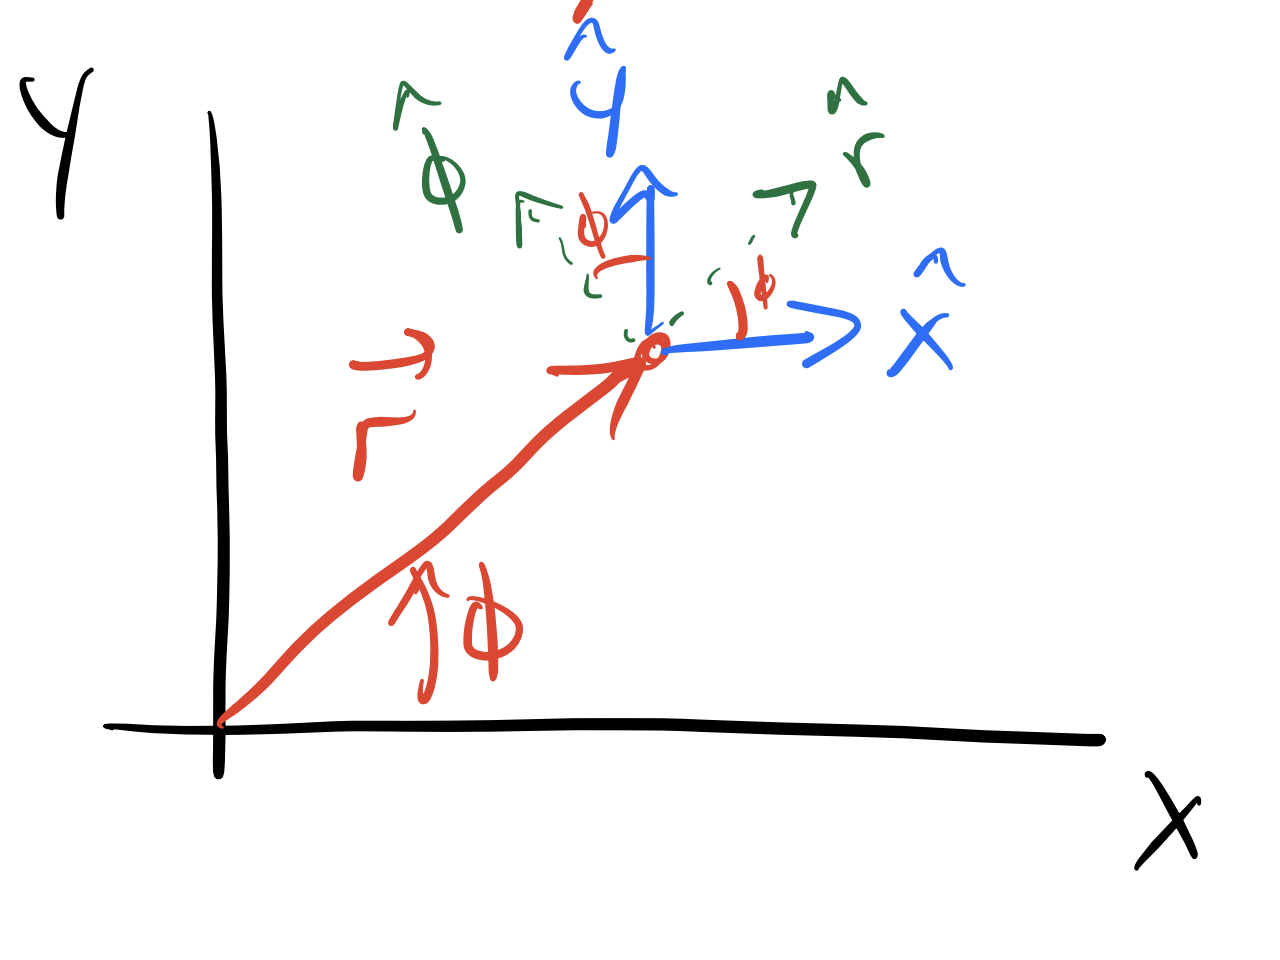
\includegraphics[keepaspectratio,alt={Position vector in polar coordinates}]{/Users/caballero/repos/teaching/modern-classical-mechanics/images/notes/week12/coordinate-system.png}}
\caption{Position vector in polar coordinates}
\end{figure}

The red arrow represents the position vector \(\vec{r}\), which is a
length \(r\) from the origin at an angle \(\phi\) from the \(x\)-axis.
At the tip of the vector we have drawn the Cartesian unit vectors
\(\hat{x}\) and \(\hat{y}\) in blue, and the polar unit vectors
\(\hat{r}\) and \(\hat{\phi}\) in green. Notice that the polar unit
vectors are rotated by an angle \(\phi\) from the Cartesian unit
vectors. We can simply write the position vector in terms of these unit
vectors as:

\[
\vec{r} = r \hat{r} \;\text{where}\; r = |\vec{r}|.
\]

We start by taking the derivative of the position vector \(\vec{r}\)
with respect to time \(t\) to find the velocity \(\vec{v}\). Using the
product and chain rules, we have:

\[
\dfrac{d\vec{r}}{dt} = \frac{d}{dt}(r \hat{r}) = \dot{r} \hat{r} + r \frac{d\hat{r}}{dt}.
\]

What is \(\frac{d\hat{r}}{dt}\)?

We note that the green unit vectors for \(\hat{r}\) and \(\hat{\phi}\)
are not constant, they change direction as the particle moves. We can
write them in terms of the Cartesian unit vectors, which do not change
with time, as follows:

\[
\hat{r} = \cos(\phi) \hat{x} + \sin(\phi) \hat{y}, \;\;\;\; \hat{\phi} = -\sin(\phi) \hat{x} + \cos(\phi) \hat{y}.
\]

Now, we differentiate \(\hat{r}\) with respect to time \(t\) using the
chain rule:

\[
\frac{d\hat{r}}{dt} = \frac{d}{dt}(\cos(\phi) \hat{x} + \sin(\phi) \hat{y}) = -\sin(\phi) \dot{\phi} \hat{x} + \cos(\phi) \dot{\phi} \hat{y} = \dot{\phi} \hat{\phi}
\]

So our expression for the velocity becomes:

\[
\vec{v} = \dot{r} \hat{r} + r \dot{\phi} \hat{\phi}.
\]

We differentiate again to find the acceleration
\(\vec{a} = \frac{d\vec{v}}{dt}\):

\[
\frac{d\vec{v}}{dt} = \frac{d}{dt}(\dot{r} \hat{r} + r \dot{\phi} \hat{\phi}) = \ddot{r} \hat{r} + \dot{r} \frac{d\hat{r}}{dt} + \dot{r} \dot{\phi} \hat{\phi} + r \ddot{\phi} \hat{\phi} + r \dot{\phi} \frac{d\hat{\phi}}{dt}
\]

Recall from above that \(\frac{d\hat{r}}{dt} = \dot{\phi} \hat{\phi}\).
Now, let's find \(\frac{d\hat{\phi}}{dt}\):

\[
\frac{d\hat{\phi}}{dt} = \frac{d}{dt}(-\sin(\phi) \hat{x} + \cos(\phi) \hat{y}) = -\cos(\phi) \dot{\phi} \hat{x} - \sin(\phi) \dot{\phi} \hat{y} = -\dot{\phi} \hat{r}
\]

Substituting these results, the acceleration becomes:

Using Newton's second law, \(\vec{a} = \vec{F}/m\), we have:

\[
\vec{F}_{net} = m\left[(\ddot{r} - r \dot{\phi}^2) \hat{r} + (2 \dot{r} \dot{\phi} + r \ddot{\phi}) \hat{\phi}\right]
\]

So the radial and angular components of the net force are:

\[
\vec{F}_{r} = m(\ddot{r} - r \dot{\phi}^2) \hat{r}
\]

\[
\vec{F}_{\phi} = m(2 \dot{r} \dot{\phi} + r \ddot{\phi}) \hat{\phi}
\]

This gives us the net force in terms of the radial and angular
components in polar coordinates.

    \subsubsection{Skateboard Example}\label{skateboard-example}

Let's see the utility of using polar coordinates by applying it to a
skateboarder moving on a circular track. In this case, the skateboarder
is constrained to move along a circular path of radius \(r\). Consider a
skateboarder moving on that circular track as shown below:

\begin{figure}
\centering
\pandocbounded{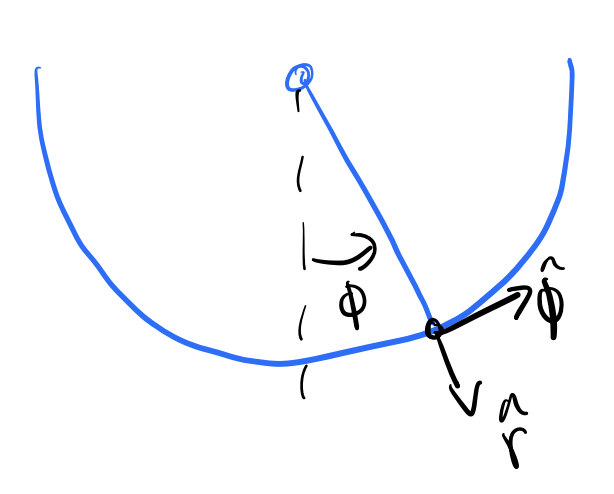
\includegraphics[keepaspectratio,alt={Skateboarder on a circular track}]{/Users/caballero/repos/teaching/modern-classical-mechanics/images/notes/week12/skateboard.png}}
\caption{Skateboarder on a circular track}
\end{figure}

At this point in the track, we can draw the free body diagram of the
skateboarder. The forces acting on the skateboarder are the Earth's
gravitational force and the normal force of the ramp.

\begin{figure}
\centering
\pandocbounded{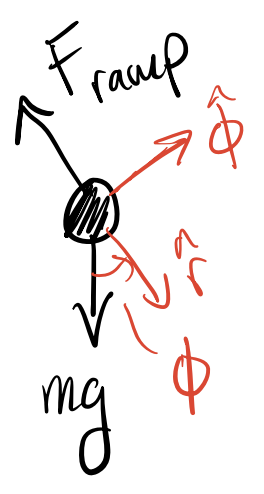
\includegraphics[keepaspectratio,alt={Free body diagram of skateboarder}]{/Users/caballero/repos/teaching/modern-classical-mechanics/images/notes/week12/skateboard-free-body.png}}
\caption{Free body diagram of skateboarder}
\end{figure}

We can use Newton's law in polar coordinates to analyze the forces
acting on the skateboarder. This is because the normal force is always
perpendicular to the surface of the ramp and will only have a radial
component in polar coordinates. Thus we need only decompose the
gravitational force into its radial and angular components.

The sum of all forces in the radial direction are given by:

\[\sum F_r = ma_r = -F_{ramp} + mg \cos(\phi) = m\left(\ddot{r} - r \dot{\phi}^2\right)\]

We note that \(r=R\), that is the radius is fixed, so

\[\ddot{r} = 0.\]

Therefore, we can simplify the equation to:

\[-F_{ramp} + mg \cos(\phi) = -mR \dot{\phi}^2.\]

In the tangential direction, we have:

\[\sum F_{\phi} = ma_{\phi} = -mg \sin(\phi) = m\left(2 \dot{r} \dot{\phi} + r \ddot{\phi}\right)\]

Because \(r=R\) is constant, we have \(\dot{r} = 0\). Thus, the equation
simplifies to:

\[-mg \sin(\phi) = mR \ddot{\phi}\]

Or, we can express this as:

\[\ddot{\phi} = -\frac{g}{R} \sin(\phi).\]

\paragraph{The Normal Force as a Function of
Time}\label{the-normal-force-as-a-function-of-time}

We can solve this equation using numerical methods to find \(\phi(t)\),
the angular position of the skateboarder as a function of time. This can
be used to then find the normal force as a function of time by
substituting \(\phi(t)\) back into the radial equation we derived above:

\[F_{ramp} = mg \cos(\phi(t)) + mR \dot{\phi}^2(t).\]

Note that this force is a
\href{https://en.wikipedia.org/wiki/Constraint_force}{force of
constraint} because it is not an external force acting on the
skateboarder but rather a force that arises from the constraint of the
circular track. These forces are important in mechanics and can be
analyzed using Lagrangian mechanics as well. They are not typically
conservative forces and do not have a potential energy associated with
them.

\paragraph{Simple Harmonic Motion}\label{simple-harmonic-motion}

If we consider small angles, i.e., \(\sin(\phi) \approx \phi\), then the
equation of motion for \(\ddot{\phi}\) becomes:

\[\ddot{\phi} \approx -\frac{g}{R} \phi.\] on (SHM) with angular
frequency \(\omega = \sqrt{\frac{g}{R}}\). Thus, for small angles, the
motion of the skateboarder on the circular track will exhibit SHM. The
solution to this equation will be:

\[\phi(t) = A \cos(\omega t) + B \sin(\omega t),\]

where \(A\) and \(B\) are constants determined by the initial conditions
of the problem.

    \subsubsection{Newton's Laws and Equations of
Motion}\label{newtons-laws-and-equations-of-motion}

So far you have studied the work of physics from the perspective of
Newtonian Mechanics, which is based on forces and their effects on
motion. The idea behind using Newton's Laws is that:

\begin{enumerate}
\def\labelenumi{\arabic{enumi}.}
\tightlist
\item
  We can identify all the interactions with a body (i.e., all the forces
  and torques acting on it).
\item
  We can write models of those interactions as mathematical expressions
  (i.e., force laws like \(\vec{F} = -k \vec{x}\) for a spring or
  \(b v^2\) for drag).
\item
  We can vectorially sum all the individual interactions to find the net
  result (i.e., \(\sum \vec{F}_i = \vec{F}_{net}\)).
\item
  We can then use Newton's second law to find the acceleration of the
  body, \(\vec{a} = \frac{\vec{F}_{net}}{m}\).
\end{enumerate}

This process has produced our
\textbf{\href{https://en.wikipedia.org/wiki/Equation_of_motion}{equations
of motion}} for a system. Which we then investigated in detail
throughout the course.

```\{admonition\} Spring Example We have solved the spring problem many
times using Newton's Laws. The spring (\(k\)) is attached to a block of
mass \(m\) on a frictionless surface. There is a dashpot connected to
the block with a damping coefficient \(b\). We know the drag force is
opposite the motion. We can write:

\[F_{spring} = -k x\]

\[F_{drag} = -b v\]

Thus, the net force on the block is:

\[F_{net} = F_{spring} + F_{drag} = -k \vec{x} - b \vec{v}\]

We can then substitute this into Newton's second law to find the
acceleration of the block:

\[a = \frac{F_{net}}{m} = -\frac{k}{m} x - \frac{b}{m} v\]

And thus our equation of motion for the block is:

\[\ddot{x} = -\frac{k}{m} x - \frac{b}{m} \dot{x}\] ```

    \subsection{Lagrangian Mechanics}\label{lagrangian-mechanics}

The Lagrangian Formulation is rooted in classical optimization, but it
is equivalent to Newton's work. However, it uses energy (a scalar) to do
so. This means we can exploit coordinate transformations that do not
change the scalar value of the energy.

Epistemologically, Lagrange's approach is an exploration of phase space
to determine paths the dynamical system can take. You can think of this
as one level of abstraction above plotting the known phase space,
because we don't yet have the equations of motion.

Let's try an example we have seen before, the spring-mass system.

\subsubsection{Example: Spring-Mass
System}\label{example-spring-mass-system}

As you will learn, to get the EOM for a non-dissipative system, we form
a function called the \textbf{Lagrangian}:

The Lagrangian is defined as:

\[
\mathcal{L} = T - V
\]

Where: - \(T\) is the \textbf{kinetic energy} of the system. - \(V\) is
the \textbf{potential energy} of the system.

For a 1D spring-mass system, we have:

\[T = \frac{1}{2} m \dot{x}^2 \quad V = \frac{1}{2} k x^2\]

Now we follow the optimization routine, which is applying the
Euler-Lagrange equations to the Lagrangian. The Euler-Lagrange equation
for \(\mathcal{L}(x,\dot{x},t)\) is given by:

\[
\frac{d}{dt} \left( \frac{\partial \mathcal{L}}{\partial \dot{x}} \right) - \frac{\partial \mathcal{L}}{\partial x} = 0.
\]

Our Lagrangian for the spring-mass system is:

\[\mathcal{L}(x, \dot{x}) = T - V = \frac{1}{2} m \dot{x}^2 - \frac{1}{2} k x^2\]

Now we can compute the necessary derivatives:

\[\frac{\partial \mathcal{L}}{\partial \dot{x}} = m \dot{x}\]
\[\frac{\partial \mathcal{L}}{\partial x} = -k x\]

Now we can substitute these into the Euler-Lagrange equation:

\[
\frac{d}{dt} \left( m \dot{x} \right) - (-k x) = 0
\]

\[m\ddot{x} + kx = 0\]

This is the same equation of motion we derived using Newton's laws for
the spring-mass system.

\[\ddot{x} = -\frac{k}{m} x\] This shows that Lagrangian mechanics can
reproduce the same equations of motion as Newtonian mechanics, but it
does so by focusing on the energy of the system rather than forces
directly.

    \subsubsection{Why does this work?}\label{why-does-this-work}

Lagrangian mechanics works because it is based on the
\href{https://en.wikipedia.org/wiki/Action_principles}{principle of
least action} (or stationary action). This principle states that the
actual path taken by a system between two points in phase space is the
one that
\href{https://en.wikipedia.org/wiki/Hamilton\%27s_principle}{minimizes
(or makes stationary) the action}, which is the integral of the
Lagrangian over time.

This is not magic, it's an application of the
\href{https://en.wikipedia.org/wiki/Calculus_of_variations}{calculus of
variations}. The action is a functional, and the Euler-Lagrange
equations provide a way to find the stationary points of that
functional. By applying these equations to the Lagrangian, we can derive
the equations of motion for a system.

We can think of this as a system that evolves in time, but does so in a
way that is optimal in some sense. The approach allows us to find the
path the system will take by exploiting
\href{https://en.wikipedia.org/wiki/Hamilton\%27s_principle}{Hamilton's
principle}: \emph{The path taken by a dynamical system between two
points in phase space is the one that minimizes the time integral of the
Lagrangian}.

Mathematically,

\[\delta \int_{t_1}^{t_2} \mathcal{L}(x(t), \dot{x}(t), t) dt = 0\]

Where \(\delta\) indicates that we are looking for a stationary point of
the action integral. This is precisely the formulation of the calculus
of variations, which allows us to find the path that minimizes (or makes
stationary) the action integral.

So, we know that the equation that will produce the \(\mathcal{L}\) that
minimizes the action integral is given by the Euler-Lagrange equations.

\[\frac{d}{dt} \left( \frac{\partial \mathcal{L}}{\partial \dot{x}} \right) - \frac{\partial \mathcal{L}}{\partial x} = 0\]

In fact, this approach holds in each Cartesian coordinate, so that the
equations of motion can be derived in any coordinate system.

\[\frac{d}{dt} \left( \frac{\partial \mathcal{L}}{\partial \dot{x}_i} \right) - \frac{\partial \mathcal{L}}{\partial x_i} = 0\]

where \(x_i\) can be \(x, y, z\) if
\(\mathcal{L}(x,y,z,\dot{x},\dot{y},\dot{z},t)\).

    \subsubsection{Generalized Coordinates}\label{generalized-coordinates}

As it turns out, our approach can make use of an phase coordinate
\((\theta, \phi, x, y, \rho, z, \ldots)\) and their first derivatives
\((\dot{\theta}, \dot{\phi}, \dot{x}, \dot{y}, \dot{\rho}, \dot{z}, \ldots)\).
In fact, we can do so for any set of
\href{https://en.wikipedia.org/wiki/Generalized_coordinates}{generalized
coordinates} that describe the configuration of a system. Generalized
coordinates are a set of coordinates that uniquely define the
configuration of a system relative to some reference configuration. We
denote them as \(q_i\) where \(i\) runs from 1 to \(n\), and their time
derivatives as \(\dot{q}_i\).

The generalized position is given by:

\[\vec{q} = (q_1, q_2, \ldots, q_n)\]

And the generalized velocity (or time derivative of the generalized
coordinates) is given by:

\[\vec{\dot{q}} = \left(\dot{q}_1, \dot{q}_2, \ldots, \dot{q}_n\right)\]

These \(N\) coordinates would give tise to a set of \(N\) equations of
motion (subject to potential reductions due to constraints). The
Lagrangian can be expressed in terms of these generalized coordinates
and velocities:

\[
\mathcal{L} = \mathcal{L}(q_1, q_2, \ldots, q_n, \dot{q}_1, \dot{q}_2, \ldots, \dot{q}_n, t)
\]

The Euler-Lagrange equations can then be applied to each generalized
coordinate \(q_i\):

\[
\frac{d}{dt} \left( \frac{\partial \mathcal{L}}{\partial \dot{q}_i} \right) - \frac{\partial \mathcal{L}}{\partial q_i} = 0, \quad i = 1, 2, \ldots, n
\]

    \subsection{Example: Plane Pendulum}\label{example-plane-pendulum}

To get some intuition for how Lagrangian mechanics works, let's consider
an example we have seen before: the plane pendulum.

A pendulum bob of mass \(m\) is attached to a fixed point by a rod of
length \(l\). The bob swings in a vertical plane under the influence of
gravity as shown below. We define \(U=0\) at the top of ceiling where
the rod is attached.

\begin{figure}
\centering
\pandocbounded{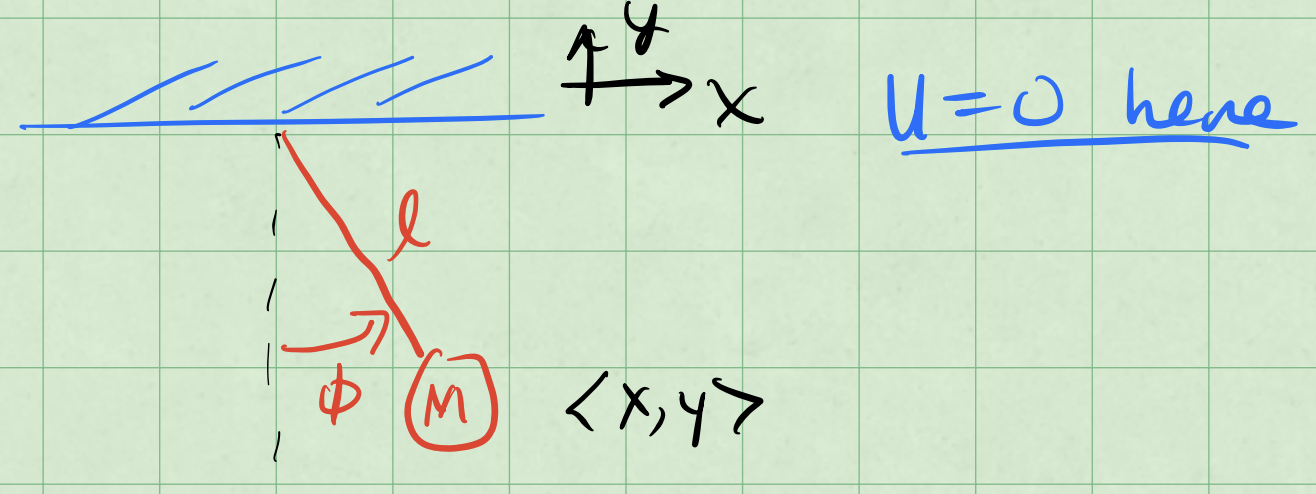
\includegraphics[keepaspectratio,alt={Pendulum Diagram}]{/Users/caballero/repos/teaching/modern-classical-mechanics/images/notes/week12/plane-pendulum.png}}
\caption{Pendulum Diagram}
\end{figure}

The location of the bob is \(\langle x, y \rangle\). We can use the
\(x,y\) coordinates to ``naively'' setup the Lagrangian and see what
happens.

The kinetic energy \(T\) of the pendulum bob is given by:

\[T(\dot{x}, \dot{y}) = \frac{1}{2} m (\dot{x}^2 + \dot{y}^2).\]

The potential energy \(V\) of the pendulum bob is given by:

\[V(x,y) = +mgy.\]

Note \(y\) is negative in the downward direction.

So we can write the Lagrangian \(\mathcal{L}\) as:

\[
\mathcal{L}(x, y, \dot{x}, \dot{y}) = T - V = \frac{1}{2} m (\dot{x}^2 + \dot{y}^2) - mgy
\]

We will get two equations of motion from the Euler-Lagrange equations,
one for \(x\) and one for \(y\). For \(x\), we have:

\[\frac{d}{dt} \left( \frac{\partial \mathcal{L}}{\partial \dot{x}} \right) - \frac{\partial \mathcal{L}}{\partial x} = 0\]
\[\frac{d}{dt} \left( m \dot{x} \right) = 0.\]

This suggests that the momentum in the \(x\)-direction
(\(p_x= m\dot{x}\)) is conserved, which cannot be correct for a
pendulum.

For \(y\), we have:

\[\frac{d}{dt} \left( \frac{\partial \mathcal{L}}{\partial \dot{y}} \right) - \frac{\partial \mathcal{L}}{\partial y} = 0\]
\[\frac{d}{dt} \left( m \dot{y} \right) - (-mg) = 0\]
\[m\ddot{y} + mg = 0\] \[\ddot{y} = -g.\]

There's no tension force? That can't be right.

\textbf{We failed to include the constraint of the pendulum!} The
pendulum is constrained to move along a circular arc of radius \(l\).
This means that the coordinates \(x\) and \(y\) are not independent, and
we cannot just use \(x,y\) as coordinates. This is a classic example of
why we need to use generalized coordinates in Lagrangian mechanics.

The constraint for the pendulum is given by:

\[x^2 + y^2 = l^2\]

This tells us that,

\[\dot{x}^2 + \dot{y}^2 = \dot{r}^2 + r^2 \dot{\phi}^2 = l^2 \dot{\phi}^2\]

where \(r=l\) is constant. So the constraint tells us that the motion of
the pendulum is constrained to a circle of radius \(l\) and it provides
a relationship between the velocities \(\dot{x}\) and \(\dot{y}\).

So as you might have guessed, we need to use a different coordinate
system to describe the motion of the pendulum. We can use \textbf{plane
polar coordinates} \((r, \phi)\) where \(r=l\) is constant and \(\phi\)
is the angle from the vertical.

\[\mathcal{L}(x, y, \dot{x}, \dot{y}) \rightarrow \mathcal{L}(r, \phi, \dot{r}, \dot{\phi})\]

The kinetic energy \(T\) in polar coordinates is given by:

\[T = \frac{1}{2} m \left( \dot{x}^2 + \dot{y}^2 \right) = \frac{1}{2} ml^2\dot{\phi}^2 = T(\dot{r}, \dot{\phi}).\]

The potential energy \(V\) becomes:

\[V = mgy = - mg l \cos(\phi) = V(r, \phi)\]

Now we can write the Lagrangian \(\mathcal{L}\) in terms of the polar
coordinates:

\[
\mathcal{L}(r, \phi, \dot{r}, \dot{\phi}) = T - V = \frac{1}{2} m l^2 \dot{\phi}^2 + mgl \cos(\phi)
\]

Notice that it is actually only a function of \(\phi\) and
\(\dot{\phi}\), because \(r=l\) is constant.

\[\mathcal{L}(l, \phi, \dot{\phi}) = \frac{1}{2} m l^2 \dot{\phi}^2 - mgl \cos(\phi)\]

Thus, we have a 1D equation of motion. This makes sense because the
pendulum is constrained to move in a circular arc, and we can describe
its motion using just one coordinate \(\phi\).

Now we can apply the Euler-Lagrange equation to find the equation of
motion for \(\phi\):

\[
\frac{d}{dt} \left( \frac{\partial \mathcal{L}}{\partial \dot{\phi}} \right) - \frac{\partial \mathcal{L}}{\partial \phi} = 0
\]

\[-mgl \sin(\phi) + \frac{d}{dt} (ml^2 \dot{\phi}) = 0\]

And thus the \(\phi\) equation of motion becomes:

\[ml^2 \ddot{\phi} + mgl \sin(\phi) = 0\]

or,

\[\ddot{\phi} = - \frac{g}{l} \sin(\phi).\]

As we have seen, for small \(\phi\), this reduces to simple harmonic
motion:

\[\ddot{\phi} \approx -\frac{g}{l} \phi \quad \text{for small } \phi.\]

    


    % Add a bibliography block to the postdoc
    
    
    
\end{document}
